% Bản dịch đầy đủ v5.1 để tác giả đọc; không áp giới hạn sáu trang.
% Dùng dấu chấm thập phân thống nhất với bản Anh và dữ liệu nguồn.
\documentclass[conference]{IEEEtran}
\IEEEoverridecommandlockouts
\usepackage{fontspec}
\setmainfont{Times New Roman}
\setsansfont{Arial}
\setmonofont{DejaVu Sans Mono}
\usepackage{graphicx}
\graphicspath{{figures/}}
\usepackage{amsmath,amssymb,booktabs,array,url,balance,microtype}

\title{Khi xác nhận của camera có lợi và có hại: Chính sách cấp quyền phanh AEB radar--camera và mức độ nghiêm trọng của thất bại trong CARLA}
\author{
\IEEEauthorblockN{Mai Việt Hoàng và Phạm Đức An}
\IEEEauthorblockA{\textit{Đại học Bách khoa Hà Nội}\\
Hà Nội, Việt Nam\\hoangmai04222@gmail.com}
}
\begin{document}
\maketitle

\begin{abstract}
Camera có thể chặn phanh nhầm do radar kích hoạt, nhưng việc không nhận diện
được xe không chứng minh rằng đường phía trước trống. Bài báo đánh giá ba
chính sách cấp quyền phanh ở cuối chuỗi xử lý---radar-only, camera gate cứng
và camera gate có radar emergency fallback---trong cùng một hệ thống từ cảm
biến đến phanh trên CARLA. Đơn vị phân tích chính là điều kiện định danh
(\emph{named condition}): 105 điều kiện core và tập hold-out bất lợi đã khóa gồm
14 điều kiện; mỗi điều kiện lặp năm lần để kiểm tra tính nhất quán, không phải
tần suất giao thông. Precision/recall trên core lần lượt là 0.913/0.988,
1.000/0.965 và 1.000/0.988. Fallback phục hồi hai tình huống vật cản không phải
xe giữa làn bị camera gate cứng chặn, đồng thời chặn tám trường hợp phanh nhầm
trước vật thể gần mép đường. Thứ hạng đảo chiều trên hold-out: camera gate cứng
đạt 11/14 điều kiện, so với 7/14 của fallback, do bốn điều kiện mục tiêu radar
ảo tổng hợp tồn tại ổn định thỏa mãn các luật khẩn cấp. Cả 20 lượt fallback với
mục tiêu ảo đều dừng dưới 1~km/h, từ tốc độ bắt đầu phanh có trung vị
78.4~km/h, thời gian phanh 3.60~s và trung vị giảm tốc cực đại
9.02~m/s$^2$. Một ghế dài chưa dùng khi phát triển cho thấy đánh đổi ngược lại:
tốc độ ở tick cuối trước va chạm là 32.57~km/h với radar-only, 54.93~km/h với
fallback và 59.95~km/h với camera gate cứng. So sánh theo cặp, loại bỏ thành
phần, nhiễu loạn có kiểm soát và log truy nguyên từ chiến dịch CUDA 2,461 lượt
đã khóa giúp xác định thất bại ở khâu hình thành track, cấp quyền và dừng xe
sau khi được cấp quyền. Đóng góp là so sánh thực nghiệm có kiểm soát về chính
sách phanh và mức độ nghiêm trọng của thất bại, không phải một cơ chế fusion
mới hay ưu thế an toàn tổng quát.
\end{abstract}
\begin{IEEEkeywords}
phanh khẩn cấp tự động, camera gate, radar emergency fallback,
phanh nhầm, chèn lỗi tổng hợp, đánh giá theo tình huống
\end{IEEEkeywords}

\section{Giới thiệu}
Phanh khẩn cấp tự động (AEB) không chỉ cần xác định có phát hiện vật thể hay
không, mà còn phải quyết định bằng chứng hiện có đã đủ để phanh kịp thời chưa.
Radar cung cấp khoảng cách và vận tốc tương đối; thông tin ngữ nghĩa của camera
có thể loại bỏ mục tiêu radar không hợp lý. Tuy nhiên, bộ nhận diện camera chỉ
có lớp xe cũng có thể từ chối cấp quyền trước vật cản thật không phải xe. Do
đó, hiệu quả AEB phụ thuộc toàn bộ chuỗi nhận thức--rủi ro--chấp hành, thay vì
chỉ độ chính xác của bộ nhận diện \cite{yang2022aebreview}.

Nghiên cứu tách riêng \emph{chính sách cấp quyền phanh ở cuối chuỗi xử lý}:
quy tắc chấp nhận hoặc phủ quyết yêu cầu phanh đã được khâu đánh giá rủi ro
radar dùng chung đưa ra. Camera gate cứng yêu cầu xác nhận bằng hình ảnh.
Emergency fallback chỉ nới quyền phủ quyết đối với track radar ổn định, gần
tâm quỹ đạo, có đủ điểm hỗ trợ và đồng thời có TTC cùng biên khoảng cách dừng
ở mức nguy hiểm. Lợi ích mong muốn là phục hồi có chọn lọc, không quay lại
phanh radar-only không bị camera hạn chế. Câu hỏi còn mở là liệu cùng quy tắc
đó có phân biệt được vật cản ngoài lớp nhận diện với mục tiêu ảo đủ thuyết
phục hay không.

Ba câu hỏi nghiên cứu là: (RQ1) điều kiện định danh nào thay đổi kết quả hệ
thống khi đổi chính sách cấp quyền; (RQ2) cơ chế thất bại nào vẫn tồn tại khi
cho phép radar vượt camera gate; và (RQ3) điều gì bị che khuất nếu đánh giá chỉ
dừng ở recall kích hoạt phanh và số va chạm? CARLA hỗ trợ thay thế thành phần
có kiểm soát và lặp lại thí nghiệm cận va chạm
\cite{dosovitskiy2017carla,kang2019testing}. Điều đó không làm cho tập tình
huống được xây dựng trở thành đại diện của giao thông đường bộ.

Các đóng góp gồm: (1) so sánh ba chính sách theo cặp, giữ chung xử lý radar,
bộ điều khiển và cách chấm điểm; (2) phân tích theo cơ chế, liên hệ quyền phủ
quyết của camera, điều kiện khẩn cấp và track bị thiếu với kết quả core cùng
hold-out bất lợi; và (3) báo cáo theo điều kiện kết hợp mức độ nghiêm trọng
của phanh nhầm và tốc độ trước va chạm, có dấu vết thực thi CUDA và artifact
đã khóa. Đây là các đóng góp thực nghiệm. Cách tổ chức và trình bày theo cặp
bổ sung trong bản sửa đổi này sử dụng lại evidence đã khóa, không đưa vào
thuật toán hay chiến dịch thí nghiệm mới.

\section{Nghiên cứu liên quan và ranh giới đóng góp}
Nhận diện xe bằng radar--camera cho AEB đã được nghiên cứu. Kim và Song xử lý
chọn nhầm mục tiêu bằng bằng chứng hình dạng và chuyển động
\cite{kim2013vehicle}; Hsu và cộng sự lọc nhiễu radar/camera, gồm các tín hiệu
liên quan đến phản xạ \cite{hsu2015noise}. Bae và cộng sự dùng fusion
LiDAR--camera để ước lượng xe gần nhất trên quỹ đạo \cite{bae2021cipv}.
Zhang và cộng sự kết hợp chọn mục tiêu trên đường cong, TTC, khoảng cách an
toàn và phanh phân tầng \cite{zhang2023curved}. Những phương pháp học máy như
CenterFusion hướng đến phát hiện vật thể 3-D \cite{nabati2021centerfusion}.
Vì vậy, bài báo không nhận xác nhận bằng camera hoặc phanh phân tầng là điểm mới.

Nghiên cứu gần nhất theo hướng xác minh là bản tiền công bố của Akula và cộng
sự \cite{akula2026radarguided}. Họ thử nghiệm xác minh mật độ biên trong vùng
ảnh do radar chỉ định trên xe có gắn thiết bị, thay vì nhận diện ngữ nghĩa
toàn ảnh. Kết quả dàn dựng báo cáo không bỏ sót phanh trong 33 phiên có nguy
cơ và có phanh ở cả ba phiên không nguy cơ tại điểm vận hành ưu tiên recall.
Điều này củng cố nhu cầu kiểm tra các can thiệp không cần thiết, nhưng không
phải baseline số liệu cho kết quả CARLA của chúng tôi: cảm biến, tốc độ,
nhãn và cách xác minh khác nhau. So sánh hẹp hơn của chúng tôi giữ cố định
chuỗi xử lý phía trước và thay ba luật cấp quyền phanh, trong đó có cơ chế
radar vượt quyền phủ quyết của gate chỉ nhận diện xe.

Đánh giá hệ thống bằng mô phỏng \cite{gomez2022carla} và các dạng cảm biến
thị giác khác cho AEB trong CARLA \cite{feng2025dvs} cũng đã có nghiên cứu.
Rao và cộng sự tái dựng các trường hợp AEB ngoài chuẩn và phân tích định lượng
thất bại \cite{rao2024corner}; bản thân kiểm thử corner case không phải tính
mới của chúng tôi. Kraus và cộng sự cung cấp dữ liệu mục tiêu radar ảo có gán
nhãn \cite{kraus2021ghost}. Khác với đa đường đo thực tế, tín hiệu tổng hợp
trong nghiên cứu này là \emph{synthetic fault injection}, tức chèn lỗi theo
thuộc tính của luật. Mức trừu tượng của mô hình radar giới hạn mạnh khả năng
chuyển kết luận từ kiểm thử ảo \cite{magosi2022radar}.

Đánh giá đe dọa theo xác suất \cite{sandblom2011threat} và ước lượng Bayesian
về xác suất tồn tại vật thể trong theo dõi radar--camera
\cite{lindenmaier2022existence} tiếp tục xác định ranh giới đóng góp. Fallback
ở đây là luật cấp quyền tất định, không phải suy luận xác suất tồn tại đã
hiệu chỉnh. Câu hỏi là luật đơn giản này được gì, mất gì và không giải quyết
được gì trong so sánh có kiểm soát từ cảm biến đến phanh. Tình huống lấy cảm
hứng từ protocol không cấu thành kiểm thử tuân thủ ISO hoặc Euro NCAP
\cite{iso15623,euroncap_aeb}.

\section{Chuỗi xử lý dùng chung và các chính sách cấp quyền}
\subsection{Cảm biến, bộ nhận diện và ranh giới thông tin}
Xe ego Tesla Model 3 hoạt động tại Town04 với bước mô phỏng đồng bộ 0.05 s.
Chỉ điểm radar và ảnh RGB được dùng để nhận thức mục tiêu trực tuyến; trạng
thái ego hỗ trợ dự đoán quỹ đạo và phanh. Quyết định phanh không truy vấn
định danh actor, nhãn thật, vận tốc thật của mục tiêu hay bounding box ground
truth. Điều phối tình huống và nhãn ngoại tuyến nằm ngoài ranh giới thông tin
này. Không dùng sự thật actor để sửa một track radar yếu.

\begin{table}[t]
\caption{Cấu hình cảm biến và bộ nhận diện dùng chung, đã khóa.}
\label{tab:setup}
\centering\scriptsize
\setlength{\tabcolsep}{3pt}
\begin{tabular}{p{0.27\columnwidth}p{0.66\columnwidth}}
\toprule Thành phần & Thiết lập\\ \midrule
Camera & RGB, 1280$\times$720, FOV $70^\circ$; $(x,z)=(0.43,1.35)$ m\\
Radar & 100 m, $30^\circ\!\times6^\circ$, 2000 điểm/s; $(x,z)=(2.53,0.48)$ m\\
Bộ nhận diện & YOLO26n ONNX \cite{ultralytics_yolo}, đầu vào 640; confidence 0.25; NMS IoU 0.50\\
Dataset & 1505/300/200 ảnh; 28/6/4 phiên thu thập train/val/test tách biệt\\
Huấn luyện & Một lớp \emph{car}; AdamW; seed 2026; tiền tố SHA-256 model \texttt{dc0a6ca1754a}\\
Thời gian & Hai cảm biến: 0.05 s; suy luận: 0.15 s; giữ xác nhận: 0.35 s; bắt buộc CUDA\\
\bottomrule
\end{tabular}
\end{table}

Bảng~\ref{tab:setup} mô tả cấu hình dùng chung. Các tập dữ liệu chứa
1872/379/264 box và 21.2/16.3/18.0\% ảnh rỗng, không có ảnh trùng hoàn toàn
giữa các tập. Tách theo phiên ngăn các frame liền kề bị chia xen kẽ vào nhiều
tập, nhưng toàn bộ vẫn nằm trong miền Town04. Precision, recall,
$\mathrm{mAP}_{50}$ và $\mathrm{mAP}_{50:95}$ trên validation lần lượt là
0.9919, 0.9642, 0.9940 và 0.9495; các chỉ số detector không xác lập hiệu quả
AEB ngoài miền. Ngoại tham số đã hiệu chuẩn chiếu mục tiêu radar được chọn
lên ảnh. Xác nhận yêu cầu điểm chiếu nằm trong một car box được giữ lại.
Nhịp suy luận và hết hạn xác nhận dùng timestamp mô phỏng, không dùng thời
gian thực của máy. Thời gian giữ 0.35 s giống nhau ở hai chính sách camera
nối các lần suy luận nhưng cho phép xác nhận cũ còn hiệu lực trong khoảng
hữu hạn.

\subsection{Rủi ro và ba gate thay thế}
Điểm radar được lọc theo khoảng cách, độ cao mặt đường và quỹ đạo độ cong
không đổi dự đoán; sau đó gom cụm theo vị trí/vận tốc và liên kết qua các
frame. Hệ thống chọn một track đã xác nhận, chưa cũ và có liên quan đến va
chạm. Với khoảng cách $d$, vận tốc tương đối radar $v_r<0$ và vận tốc ego
$v_e$,
\begin{equation}
v_c=-v_r,\qquad \mathrm{TTC}=d/v_c,\qquad v_t=\max(0,v_e+v_r).
\end{equation}
Khoảng cách dừng yêu cầu và biên khoảng cách được tính bởi
\begin{equation}
d_{\rm req}=\max\!\left(d_0,v_et_r+\frac{v_e^2}{2a_e}-\frac{v_t^2}{2a_t}+d_0\right),
\quad m=d-d_{\rm req},
\end{equation}
trong đó $t_r=0.20$ s, $a_e=8$, $a_t=6$ m/s$^2$ và $d_0=1$ m là tham số
rủi ro mô phỏng. Bộ staged PID dùng chung tạo lệnh phanh liên tục.

Gọi $B_r$ là yêu cầu AEB từ radar, $C$ là xác nhận camera hiện tại, $H$ là
xác nhận còn được giữ, và $E_r$ là điều kiện khẩn cấp bao gồm trạng thái chốt
(latch). Các chính sách cấp quyền là
\begin{align}
 B_{\rm radar}&=B_r,\\
 B_{\rm hard}&=B_r\land(C\lor H),\\
 B_{\rm fallback}&=B_r\land(C\lor H\lor E_r).
\end{align}
Một lần chấp nhận khẩn cấp mới yêu cầu track đã xác nhận/chưa cũ, tuổi và
chuỗi hit $\geq3$, ít nhất sáu điểm, confidence của track $\geq0.70$, độ lệch
quỹ đạo tuyệt đối $\leq0.65$ m, TTC $\leq1.10$ s \emph{và} biên
$m\leq-2.0$ m. TTC và biên khoảng cách phải đồng thời thỏa mãn, không phải
hai lựa chọn thay thế. Sau khi được chấp nhận, fallback được chốt tới khi
radar rời \texttt{BRAKE}. Confidence ở đây là điểm số của tracker, không phải
xác suất tồn tại vật lý đã hiệu chỉnh.

Mọi gate đều cần $B_r$: car box riêng lẻ không tạo được rủi ro động học.
Radar-only vì vậy là tham chiếu không bị camera hạn chế cho cùng yêu cầu
radar. Fallback không phải radar-only, vì khi thiếu xác nhận camera nó có thể
chặn yêu cầu đó tới khi các điều kiện khẩn cấp chặt hơn được thỏa mãn.
Thứ tự xử lý là cập nhật quỹ đạo ego, track, mục tiêu, rủi ro radar, suy luận
camera theo lịch, cấp quyền và chấp hành; sau đó ghi trạng thái mô phỏng kế tiếp.

Với cùng trạng thái đầu vào, các phương trình cho
$B_{\rm hard}\leq B_{\rm fallback}\leq B_{\rm radar}$ đối với quyền phanh
Boolean. Đây là tính chất của luật, không bảo đảm tập kết quả vòng kín
lồng nhau: lịch sử phanh khác nhau làm thay đổi tốc độ, quan sát cảm biến
sau đó và thời điểm vượt ngưỡng. Vì vậy so sánh theo cặp dùng các điều kiện
được thực thi riêng, không dùng phát lại phản thực tế với giả định quan sát
tương lai giống nhau sau những hành động phanh khác nhau.

\section{Protocol, nhãn và phân tích}
\subsection{Thực thi đã khóa và các bộ tình huống được xây dựng}
Ngưỡng, suite và protocol được gắn tag repository trước khi thực thi hold-out,
tại \texttt{safe-fallback-eval-v1}. Các tình huống bất lợi được thiết kế khi
đã biết luật; kết quả của chúng không được dùng để chọn hoặc chỉnh lại
ngưỡng. Đây là \emph{hold-out cơ chế bất lợi đã khóa}, không phải mẫu mù từ
phân bố triển khai. Thống kê theo điều kiện và severity được suy ra hậu nghiệm
từ log đã khóa; không được nhầm chúng với đầu ra mới đã đăng ký trước.

Chiến dịch gồm 2,461 lượt chạy trong 639 phiên CARLA tách biệt. Các lượt lặp
của một điều kiện chạy xong trước khi chuyển sang tiến trình server mới.
Cả hai chính sách camera bắt buộc dùng \texttt{CUDAExecutionProvider}; sai
provider hoặc lỗi suy luận là điều kiện dừng kỹ thuật bắt buộc. Lượt FAIL do
thuật toán nhưng đã chạy hoàn chỉnh phải được giữ; chỉ thực thi không hoàn
chỉnh về kỹ thuật mới được phép chạy lại.

Core gồm 66 điều kiện tốc độ--khoảng cách thuộc CCRm, CCRb, cut-in và các
giới hạn liên quan; 29 điều kiện regression hỗn hợp có xe/âm tính; tám vật
thể lệch ngang gần mép; và hai vật cản box/barrel giữa làn: tổng cộng 105 điều
kiện. Sáu điều kiện lỗi tổng hợp yếu bốn điểm được đánh giá riêng, không nằm
trong ma trận nhầm lẫn core chính. Hai mươi nhiễu loạn cục bộ thay đổi tốc độ
$\pm2$ km/h, khoảng cách $\pm1$ m, thời điểm cut-in $\pm0.1$ s hoặc vị trí
vật thể $\pm0.15$ m. Mười điều kiện tắt detector loại bỏ toàn bộ detection
camera; đây là mất phát hiện hoàn toàn, không phải phân bố thời tiết tự nhiên.

Hold-out bất lợi gồm 14 điều kiện: ba loại vật thể mới giữa làn, bốn biến thể
ngoại hình xe, hai vật thể gần mép và năm hình học mục tiêu ảo tổng hợp tồn
tại ổn định với 6--10 điểm được chèn. Core và hold-out lặp năm lần; development
và perturbation lần lượt lặp hai và ba lần. Seed 2026 được ghi lại. Kết quả
hệ thống theo điều kiện được báo cáo nhất quán toàn PASS hoặc toàn FAIL qua
các lần lặp. Lặp lại đo tính nhất quán, không phải các lần gặp giao thông độc lập.

\subsection{Dự đoán phanh, thành công hệ thống và severity}
YAML đã khóa cung cấp nhãn phanh/va chạm mong đợi. Dự đoán có phanh nghĩa là
ít nhất một tick ghi \texttt{aeb\_override=true}; có va chạm nghĩa là một tick
bất kỳ ghi \texttt{collision\_count>0}. PASS hệ thống yêu cầu kết quả phanh và
va chạm khớp kỳ vọng. Trường hợp dương tính không mong đợi va chạm còn cần
khoảng cách cản trước tối thiểu $\geq0.5$ m, cùng các ràng buộc làn/mục tiêu
nếu được chỉ định. Vì vậy TP về phanh vẫn có thể va chạm hoặc vi phạm khoảng
cách dừng.

Bài báo trình bày TP/FP/TN/FN, precision/recall, PASS và số va chạm theo điều
kiện định danh. Ma trận theo cặp ghép đúng cùng định danh điều kiện. Khoảng
Wilson là khoảng tham chiếu nhị thức mang tính mô tả, tính từ số điều kiện;
không phải bảo đảm độ phủ hay suy luận quần thể giao thông cho lưới phi ngẫu
nhiên này. Không kiểm định ý nghĩa thống kê bằng cách coi lần lặp là mẫu độc
lập. Tỷ lệ lớp được thiết kế ảnh hưởng precision, và mẫu số hold-out nhỏ giới
hạn diễn giải.

Nhãn phản ánh nhu cầu phanh dự kiến trong từng điều kiện được xây dựng,
không phải việc YOLO dự đoán lớp \emph{car}. Vật cản không phải xe ở giữa
làn vì vậy là nguy cơ dương tính dù nằm ngoài không gian nhãn detector;
ghost tổng hợp không có nguy cơ vật lý là âm tính dù track radar ổn định.
Các nhãn cho phép đánh giá riêng sự phủ quyết ngữ nghĩa và tính liên quan
của nguy cơ vật lý. Tổng hợp theo điều kiện cũng giữ các dạng thất bại
riêng: thiếu khoảng cách, không phanh và va chạm không thể hoán đổi;
PASS rate bằng nhau không nhất thiết có thời điểm phanh giống nhau.

Tốc độ trước va chạm là tốc độ ego được ghi cuối cùng trước va chạm đầu tiên,
là đại lượng đại diện theo bước 0.05 s thay vì tốc độ đúng thời điểm tiếp xúc.
Thời gian phanh nhầm đếm các tick có override; giảm tốc cực đại loại trừ
khởi tạo, tick dưới 1 km/h và tick va chạm. Bài báo cũng báo cáo tốc độ/khoảng
cách khi bắt đầu phanh và việc ego có dừng dưới 1 km/h hay không. Trung vị
qua lần lặp mô tả thực thi, không phải mức độ nghiêm trọng trong quần thể.
Khi chưa có mô hình người ngồi trong xe hoặc xe đi phía sau, đây là đại lượng
động học, không phải ước lượng chấn thương hay nguy cơ va chạm thứ cấp.

\section{Kết quả: Lợi ích, phản ví dụ và mức độ nghiêm trọng}
\subsection{Các điểm vận hành theo cặp}
Bảng~\ref{tab:primary} và Hình~\ref{fig:primary} trình bày core và hold-out.
Fallback đạt 101/105 điều kiện core, so với 99 của camera gate cứng và 93 của
radar-only. Cả hai chính sách camera chặn tám trường hợp phanh nhầm do vật
thể gần mép (bốn loại vật thể, mỗi loại ở hai độ lệch ngang). Radar-only và
fallback phanh ở cả hai vật cản box/barrel giữa làn; gate cứng phủ quyết và
tạo thêm hai điều kiện FN/va chạm. Cả ba cùng có một FN tại biên hành lang
của cut-out muộn và ba điều kiện va chạm ở tốc độ cao. Do đó số điều kiện va
chạm core theo thứ tự chính sách là 3/5/3, hay 15/25/15 lượt lặp.

\begin{table*}[t]
\caption{Kết quả chính theo điều kiện định danh. CI: khoảng Wilson tham chiếu 95\% trên lưới được xây dựng; Coll.: số điều kiện va chạm.}
\label{tab:primary}
\centering\scriptsize
\setlength{\tabcolsep}{3pt}
\begin{tabular}{llrrrrrccrr}
\toprule Phạm vi & Chính sách & N & TP & FP & TN & FN & Precision [CI] & Recall [CI] & PASS & Coll.\\
\midrule
Core & Radar & 105 & 84 & 8 & 12 & 1 & .913 [.838,.955] & .988 [.936,.998] & 93 & 3\\
 & Hard & 105 & 82 & 0 & 20 & 3 & 1.000 [.955,1] & .965 [.901,.988] & 99 & 5\\
 & Fallback & 105 & 84 & 0 & 20 & 1 & 1.000 [.956,1] & .988 [.936,.998] & 101 & 3\\
\midrule
Hold-out & Radar & 14 & 6 & 5 & 2 & 1 & .545 [.280,.787] & .857 [.487,.974] & 6 & 3\\
 & Hard & 14 & 5 & 0 & 7 & 2 & 1.000 [.566,1] & .714 [.359,.918] & 11 & 3\\
 & Fallback & 14 & 6 & 4 & 3 & 1 & .600 [.313,.832] & .857 [.487,.974] & 7 & 3\\
\bottomrule
\end{tabular}
\end{table*}

Bảng~\ref{tab:paired} làm rõ thay đổi bị che khuất bởi tỷ lệ tổng hợp. Trên
core, gate cứng đạt thêm tám điều kiện nhưng mất hai so với radar; fallback
giữ được cả hai phần phục hồi. Trên hold-out, gate cứng đạt thêm bốn điều
kiện so với fallback và không mất điều kiện nào xét PASS nhị phân. Cả ba vẫn
va chạm với ba vật thể giữa làn. Điều này không có nghĩa mức giảm nhẹ hậu
quả bằng nhau, như kết quả ghế dài bên dưới cho thấy.

\begin{table}[t]
\caption{Kết quả hệ thống theo cặp điều kiện. Các cột xét chính sách A/B, không phải TP/FP về phanh.}
\label{tab:paired}
\centering\scriptsize
\setlength{\tabcolsep}{3pt}
\begin{tabular}{llrrrr}
\toprule Phạm vi & A / B & Cùng PASS & Chỉ A & Chỉ B & Cùng FAIL\\ \midrule
Core & Radar / Hard & 91 & 2 & 8 & 4\\
 & Radar / Fallback & 93 & 0 & 8 & 4\\
 & Hard / Fallback & 99 & 0 & 2 & 4\\
Hold-out & Radar / Hard & 6 & 0 & 5 & 3\\
 & Radar / Fallback & 6 & 0 & 1 & 7\\
 & Hard / Fallback & 7 & 4 & 0 & 3\\
\bottomrule
\end{tabular}
\end{table}

Cả sáu điều kiện lỗi bốn điểm yếu riêng biệt đều gây phanh nhầm ở radar-only
và bị cả hai chính sách camera chặn. Ngược lại, fallback chấp nhận bốn trong
năm mục tiêu ảo hỗ trợ cao của hold-out, chỉ chặn điều kiện lệch 0.75 m.
Các biến thể ngoại hình xe không phân biệt gate cứng với fallback vì vẫn
thuộc không gian nhãn camera. Thứ hạng chính sách thay đổi theo cơ chế có
mặt trong suite, không chỉ theo số lượt thực thi lặp lại.

\begin{figure*}[t]
\centering
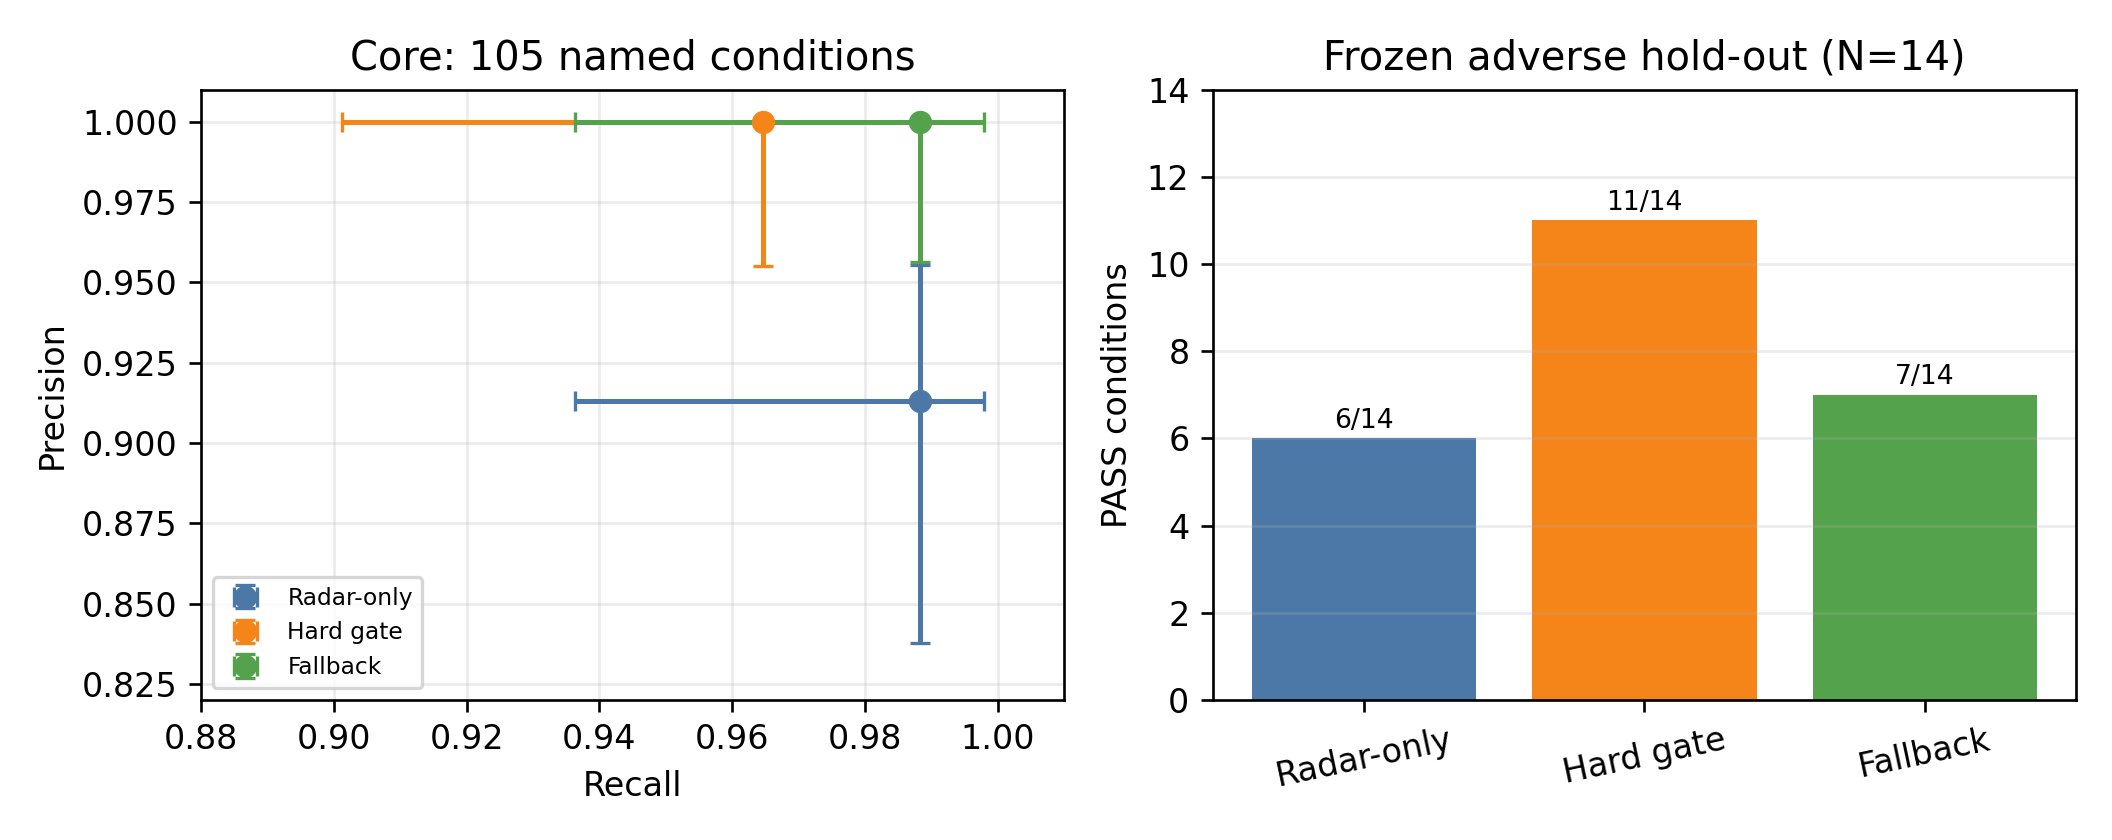
\includegraphics[width=0.90\textwidth]{scenario_level_tradeoff.png}
\caption{Evidence theo điều kiện đã khóa. Trái: precision--recall core và khoảng Wilson mô tả. Phải: PASS hệ thống trên hold-out bất lợi 14 điều kiện. Không lưới nào ước lượng tần suất giao thông thực. Hình giữ nhãn tiếng Anh để đối chiếu với bản nộp.}
\label{fig:primary}
\end{figure*}

\subsection{Cơ chế ở các khâu khác nhau của chuỗi xử lý}
\emph{Thiếu track.} Xe đẩy hàng trong hold-out tạo tối đa hai điểm ứng viên
trên quỹ đạo và không tạo cụm được xác nhận. Không yêu cầu phanh radar nào
đến gate; cơ chế cấp quyền muộn không thể phục hồi thất bại ở khâu trước
này. Cả ba va chạm mà không phanh, với trung vị tốc độ đại diện 49.96 km/h.

\emph{Phủ quyết ngữ nghĩa và cấp quyền muộn.} Ghế dài tạo track radar nhưng
không có xác nhận car dùng được. Radar-only phanh tại 12.624 m; fallback đủ
điều kiện tại 4.295 m; camera gate cứng không phanh.
Bảng~\ref{tab:severity} ghi tốc độ trước va chạm lần lượt 32.57, 54.93 và
59.95 km/h. Fallback phục hồi TP về phanh, không phục hồi dừng kịp thời.
So với gate cứng, radar-only giảm đại lượng tốc độ này khoảng 27.4 km/h,
trong khi fallback chỉ giảm 5.0 km/h.

\emph{Va chạm dù đã được cấp quyền.} Với vật thể cảnh báo giao thông, cả ba
chính sách phanh tại 21.871 m; log chính sách camera cho thấy camera xác
nhận thay vì fallback. Cả ba va chạm tại 7.82 km/h. Log xác lập rằng quyền
phanh đã được cấp, nhưng không tự xác định được lỗi động lực học tiếp xúc
hay bộ điều khiển. Trường hợp này cho thấy giảm nhẹ hậu quả bị che khuất
bởi chỉ số va chạm nhị phân.

\emph{Track giả đủ thuyết phục.} Chèn sáu điểm giữa quỹ đạo tạo track được
xác nhận trước hoặc tại 0.15 s, confidence 1.0, TTC 0.89 s và biên
$-15.21$ m. Radar-only và fallback yêu cầu phanh khẩn cấp; gate cứng không có
xác nhận car. Ghost tám và mười điểm ở tâm/độ lệch 0.50 m có hành vi tương
tự. Dịch điểm chèn tới 0.75 m vượt biên fallback 0.65 m đã khóa nhưng không
ngăn radar-only phanh. Đây là phản ví dụ tổng hợp đối với tính đầy đủ của
luật khẩn cấp, không phải phép đo tần suất ghost thực.

\begin{table}[t]
\caption{Severity hold-out: trung vị năm lượt cho mỗi điều kiện vật thể; hàng ghost tổng hợp 25/20 lượt. Tốc độ trước va chạm là đại lượng đại diện tick cuối.}
\label{tab:severity}
\centering\scriptsize
\setlength{\tabcolsep}{3pt}
\begin{tabular}{llrr}
\toprule Cơ chế & Chính sách & Bắt đầu / gap & Kết quả severity\\ \midrule
Xe đẩy & Tất cả & không phanh & 49.96 km/h trước va chạm\\
Ghế dài & Radar & 12.624 m & 32.57 km/h trước va chạm\\
 & Hard & không phanh & 59.95 km/h trước va chạm\\
 & Fallback & 4.295 m & 54.93 km/h trước va chạm\\
Cảnh báo & Tất cả & 21.871 m & 7.82 km/h trước va chạm\\
\midrule
Ghost FP & Radar (25 lượt) & 78.4 km/h & 3.60 s / 9.02 m/s$^2$\\
 & Fallback (20) & 78.4 km/h & 3.60 s / 9.02 m/s$^2$\\
\bottomrule
\end{tabular}
\end{table}

Mỗi lần phanh nhầm trước ghost đều dừng xe mô phỏng dưới 1 km/h, không phải
xung phanh một tick. Hàng ghost trình bày tốc độ bắt đầu, thời gian override
và giảm tốc cực đại; các quan sát này làm rõ ý nghĩa vận hành của suy giảm
precision trong mô phỏng. Chúng không định lượng chấn thương hoặc nguy cơ
xe sau đâm vào. FN cut-out muộn dùng chung và va chạm ở giới hạn dừng tốc
độ cao là nhóm khác: không thể coi chúng là bằng chứng camera phủ quyết,
vì radar-only cũng thất bại.

\subsection{Loại bỏ thành phần, nhiễu loạn và mất phát hiện}
Trong ablation development 12 điều kiện (hai lần lặp), fallback đầy đủ đạt
12/12. Gate cứng và biến thể không latch đều không đạt hai điều kiện
box/barrel giữa làn. Bỏ ràng buộc quỹ đạo thêm ba điều kiện phanh nhầm vật
thể gần mép; bỏ số điểm tối thiểu thêm hai điều kiện phanh nhầm ghost yếu.
Bỏ stability/confidence hoặc đổi TTC-AND-margin thành OR không thay kết quả
trên lưới tập trung này. Vì vậy tính cần thiết độc lập của chúng chưa được
xác lập. Sáu điều kiện sensitivity một yếu tố cho thấy một phanh nhầm khi
hạ số điểm và một vật cản giữa làn bị bỏ sót khi siết stability hoặc TTC.
Không tuyên bố tìm được tối ưu toàn cục.

\begin{table}[t]
\caption{Kết quả mở rộng theo điều kiện định danh, không theo lượt lặp.}
\label{tab:extended}
\centering\scriptsize
\setlength{\tabcolsep}{3pt}
\begin{tabular}{llrrrrrr}
\toprule Suite & Chính sách & Pass/N & TP & FP & TN & FN & Coll.\\ \midrule
Perturb. & Radar & 19/20 & 20 & 0 & 0 & 0 & 1\\
 & Hard & 15/20 & 15 & 0 & 0 & 5 & 5\\
 & Fallback & 18/20 & 20 & 0 & 0 & 0 & 1\\
\midrule
Camera off & Hard & 4/10 & 0 & 0 & 4 & 6 & 6\\
 & Fallback & 8/10 & 6 & 0 & 4 & 0 & 2\\
\bottomrule
\end{tabular}
\end{table}

Bảng~\ref{tab:extended} tách hai thất bại perturbation: fallback va chạm ở
gap box 19 m, nhưng tránh va chạm ở 21 m và dừng tại 0.353 m, nhỏ hơn
ngưỡng PASS 0.5 m. Đồng nhất mọi FAIL với va chạm là sai. Khi tắt detection,
fallback phanh ở cả sáu điều kiện dương tính nhưng va chạm ở hai điều kiện.
Bốn PASS của gate cứng đều là âm tính, không phải ứng phó thành công với
nguy cơ. Các phép thử cục bộ cho thấy phụ thuộc vào luật, không chứng minh
độ bền vững qua map, thời tiết hoặc lỗi cảm biến ngẫu nhiên.

\subsection{Tính toán và khả năng tái lập}
Trong 474 phiên bắt buộc CUDA có 74,928 lần suy luận và không có lỗi suy
luận. Trung vị theo phiên của p50/p95 là 9.95/11.53 ms; trung bình có trọng
số theo số lần suy luận là 11.56 ms. Mỗi tiến trình mới có một lần khởi động
nguội trên 150 ms; cực đại là 276.10 ms. Đây là thời gian ONNX đo trên máy
chủ, không gồm radar, truyền dữ liệu, điều khiển, hiển thị và chấp hành;
không phải deadline end-to-end của ECU.

Manifest phiên ghi commit, seed, phiên bản CARLA, hash model/config, provider
cấu hình/thực tế, số suy luận và lỗi. Log tick giữ số điểm hỗ trợ track,
confidence, TTC, biên khoảng cách, lý do gate, override và va chạm. Khóa
checkpoint là (định danh scenario, chỉ số lần chạy); phục hồi kỹ thuật không
được biến FAIL thuật toán thành lần retry thành công được lựa chọn.
Ma trận theo điều kiện, kết quả theo cặp và severity được tái tạo từ log đã
khóa mà không thêm hay bỏ lượt chạy. Refactor repository và thay đổi
launcher diễn ra sau đó, không phải đóng góp thí nghiệm hoặc kiểm chứng mới
cho các chính sách này.

Mã nguồn và evidence được tuyển chọn được lập chỉ mục tại
\url{https://github.com/mvhoang92/aeb}; bản đồ nguồn đi kèm xác định archive
log đã khóa, script suy ra chỉ số và checksum. Chạy lại cần cài CARLA tương
thích, model cục bộ và môi trường CUDA. Hash xác lập định danh artifact,
không bảo đảm hành vi giống từng bit trên mọi phần cứng. Phân biệt nguồn
gốc rất quan trọng: regression của phần mềm về sau không làm tăng mẫu
khoa học hoặc thay thế chiến dịch đã lưu.

\section{Thảo luận và giới hạn giá trị kết luận}
\subsection{Điều so sánh này xác lập}
Kết quả tách ba câu hỏi: radar có tạo mục tiêu không, chính sách có cho phanh
không, và hành động đã được cấp quyền có giảm nhẹ hậu quả đủ hay không?
Gộp cả ba thành một tỷ lệ thành công che khuất cả cấp quyền muộn ở ghế dài
lẫn va chạm tốc độ thấp ở vật thể cảnh báo. Tương tự, luật khẩn cấp cải
thiện recall core nhưng chấp nhận ghost có cùng thuộc tính đạt điều kiện.
Track tồn tại bền và nhiều điểm hỗ trợ làm mạnh một ước lượng mà không tự
chứng minh có vật cản vật lý.

Đây là giới hạn của thông tin và ngưỡng được thử, không phải định lý bất khả
thi cho radar--camera fusion. Gate cứng có lợi hơn theo PASS hold-out nhị
phân ở đây nhưng không theo mức giảm nhẹ va chạm ghế dài; fallback có lợi
trên core nhưng phanh nhầm hold-out đều dừng hẳn xe. Bài báo không chỉ định
chính sách phổ quát bằng cách tự gán trọng số cho các hậu quả khác loại.
So sánh tiếp theo cần có xác minh camera không phụ thuộc lớp và soft gate
được so ở mức confidence tương ứng trước khi quy lợi ích cho một thuật
toán fusion mới. Phương pháp xác suất cần hiệu chỉnh và bằng chứng vượt ra
ngoài việc đổi tên điểm tracker thành xác suất
\cite{sandblom2011threat,lindenmaier2022existence}.

Câu trả lời cho RQ1--RQ3 có điều kiện nhưng hữu ích cho thiết kế. Lợi ích
của chính sách có thể truy về một số cơ chế được xác định thay vì gọi chung
là ``fusion tốt hơn''. Cơ chế vượt gate không sửa được việc thiếu track ở
khâu trước; ngưỡng chất lượng radar vừa có thể nhận ghost vừa trì hoãn
vật cản thật. Cuối cùng, tránh va chạm, giảm nhẹ va chạm và hạn chế can thiệp
không cần thiết là các mục tiêu khác nhau. Không nên chọn chính sách chỉ
từ F1 hoặc PASS tổng hợp khi chưa xác định điều kiện vận hành và chi phí
sai sót chấp nhận được. Suite hiện tại hỗ trợ so sánh trong lưới của nó,
không ước lượng chi phí cho triển khai cụ thể.

\subsection{Giới hạn của evidence}
Thí nghiệm chỉ có một map, nền tảng ego, seed cố định, hình ảnh thuận lợi
và detector một lớp xe trong miền. Các lần lặp tương quan; hold-out 14 điều
kiện được chủ động xây dựng khi biết luật. Nó kiểm tra cơ chế bất lợi,
không phải tổng quát hóa không thiên lệch. Radar mức điểm của CARLA không
tái hiện đầy đủ vật lý đa đường; chèn lỗi không ước lượng tần suất radar
ghost thực \cite{kraus2021ghost,magosi2022radar}. Tick cuối trước va chạm có
rời rạc hóa 0.05 s và động học phanh nhầm không phải chi phí chấn thương.
Chưa có sweep nhiều map/thời tiết/ma sát, thí nghiệm cảm biến thật, HIL,
chứng minh functional safety hay chứng nhận theo tiêu chuẩn.

Cũng chưa có baseline soft gate được ghép tương ứng, không phụ thuộc lớp,
học máy hoặc xác suất. Giới hạn camera phủ quyết phụ thuộc không gian nhãn
chỉ gồm xe đã chọn, không phải kết luận về mọi hệ thống camera. Baseline
mở rộng cần protocol phát triển/đánh giá mới; hold-out đã xem có thể giữ làm
dữ liệu regression nhưng không còn là evidence kiểm thử chưa từng thấy.
Ràng buộc này bảo toàn kết quả bất lợi hiện tại thay vì chỉnh ngưỡng để
xóa các phản ví dụ.

\section{Kết luận}
Trong một hệ thống CARLA cố định, emergency fallback phục hồi hai nguy cơ
core bị camera phủ quyết và vẫn chặn phanh nhầm do vật thể gần mép. Bốn điều
kiện ghost tổng hợp tồn tại ổn định đảo ngược lợi thế của nó so với camera
gate cứng trên hold-out bất lợi. Phanh nhầm dừng hẳn và giảm nhẹ va chạm
ghế dài bị muộn cho thấy recall phanh cùng số va chạm riêng lẻ là chưa đủ.
Evidence hỗ trợ so sánh chính sách cấp quyền theo cơ chế và severity,
không hỗ trợ ưu thế fusion tổng quát. Thiếu xác nhận camera không chứng
minh đường trống, và radar có hỗ trợ ổn định không chứng minh có nguy cơ
vật lý.

\balance
\bibliographystyle{IEEEtran}
\bibliography{references}
\end{document}
